\documentclass[border=3pt]{standalone}
% Preâmbulo compartilhado pelos diagramas TikZ da aula 4 de Navegação (Representação de Mapas)
\usepackage[T1]{fontenc}
\usepackage[utf8]{inputenc}
\usepackage{lmodern}
\usepackage{amsmath}
\usepackage{xcolor}
\usepackage{tikz}
\usetikzlibrary{arrows.meta,angles,quotes,decorations.pathmorphing,decorations.pathreplacing,calc,
                positioning,shapes.geometric,shapes.misc,backgrounds,fit,
                math}

% Paleta (mesma dos SVGs originais)
\definecolor{dblue}{HTML}{2A5B8C}
\definecolor{dorange}{HTML}{B3541E}
\definecolor{dgreen}{HTML}{4A7C59}
\definecolor{dred}{HTML}{9C4B4B}
\definecolor{dcream}{HTML}{F4F1EA}
\definecolor{dshade}{HTML}{DDD7C9}

% Função gaussiana (não normalizada por padrão de escala visual)
\pgfmathdeclarefunction{gauss}{3}{%
  \pgfmathparse{1/(#3*sqrt(2*pi))*exp(-((#1-#2)^2)/(2*#3^2))}%
}

% Estilos comuns (prefixo d... para não colidir com chaves internas do pgf)
\tikzset{
  >={Stealth[length=2mm]},
  dguide/.style={gray!55, dashed, line width=0.4pt},
  daxis/.style={gray!60, line width=0.7pt, ->},
  dbody/.style={fill=black!3, draw=black!80, line width=1pt},
  dacc/.style={draw=dblue, line width=1pt},
  dlbl/.style={black!55, font=\small},
  dsub/.style={black!45, font=\footnotesize},
  dstate/.style={circle, draw=black!80, fill=dcream, line width=1pt,
                 minimum size=17mm, font=\large, inner sep=1pt},
  dobs/.style={circle, draw=black!80, fill=dshade, line width=1pt,
               minimum size=14mm, font=\large, inner sep=1pt},
  dbox/.style={rounded corners=2pt, draw=black!80, fill=dcream, line width=1pt,
               align=center, inner sep=6pt},
  dop/.style={circle, draw=black!80, fill=white, line width=1pt,
              minimum size=6mm, inner sep=0pt, font=\small},
  dtrans/.style={->, dblue, line width=1pt},
  dmeas/.style={->, dorange, line width=1pt},
  dcurve/.style={line width=1pt, dblue},
  dcurveb/.style={line width=1.4pt, dorange},
}

\begin{document}
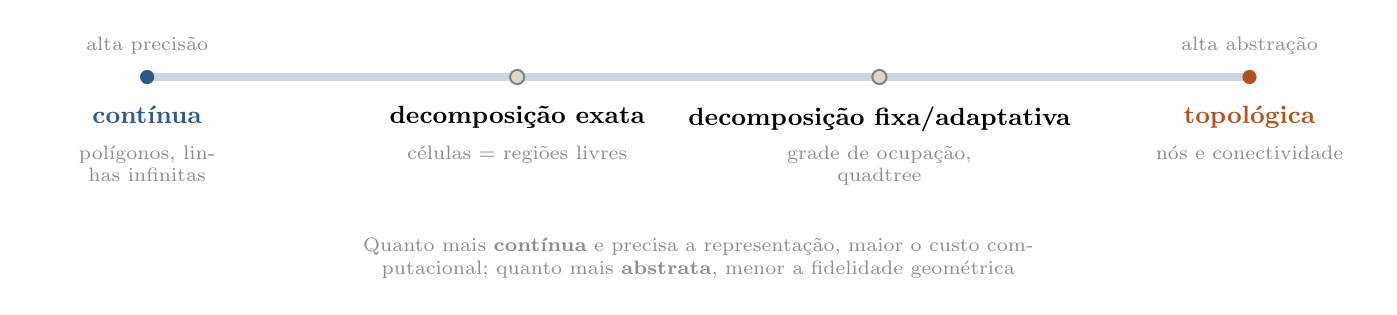
\begin{tikzpicture}[x=1cm,y=1cm]

  \draw[dcurve, line width=3pt, dblue!25] (0,0) -- (14,0);
  \fill[dblue] (0,0) circle (0.09);
  \fill[dorange] (14,0) circle (0.09);

  \node[font=\bfseries\small, dblue, anchor=north] at (0,-0.25) {contínua};
  \node[dsub, font=\scriptsize, align=center, text width=2.8cm, anchor=north] at (0,-0.75)
     {polígonos, linhas infinitas};

  \fill[dshade, draw=black!50, line width=0.7pt] (4.7,0) circle (0.09);
  \node[font=\bfseries\small, anchor=north] at (4.7,-0.25) {decomposição exata};
  \node[dsub, font=\scriptsize, align=center, text width=2.8cm, anchor=north] at (4.7,-0.75)
     {células = regiões livres};

  \fill[dshade, draw=black!50, line width=0.7pt] (9.3,0) circle (0.09);
  \node[font=\bfseries\small, anchor=north] at (9.3,-0.25) {decomposição fixa/adaptativa};
  \node[dsub, font=\scriptsize, align=center, text width=3.0cm, anchor=north] at (9.3,-0.75)
     {grade de ocupação, quadtree};

  \node[font=\bfseries\small, dorange, anchor=north] at (14,-0.25) {topológica};
  \node[dsub, font=\scriptsize, align=center, text width=2.8cm, anchor=north] at (14,-0.75)
     {nós e conectividade};

  \node[dsub, font=\scriptsize] at (0,0.4) {alta precisão};
  \node[dsub, font=\scriptsize] at (14,0.4) {alta abstração};

  \node[dsub, font=\scriptsize, align=center, text width=15.5cm] at (7,-2.3)
     {Quanto mais \textbf{contínua} e precisa a representação, maior o custo computacional; quanto mais \textbf{abstrata}, menor a fidelidade geométrica};

\end{tikzpicture}
\end{document}
